\documentclass{article}

\usepackage{amsmath}
\usepackage{graphicx}
\usepackage{listings}
\usepackage{color}


\usepackage{xepersian}
\settextfont{BNazanin} 
\linespread{1.3}
\newcommand{\linia}{\rule{\linewidth}{0.5pt}}

\def\LOGO{
\begin{picture}(0,0)\unitlength=1cm
\put (0.5,0) {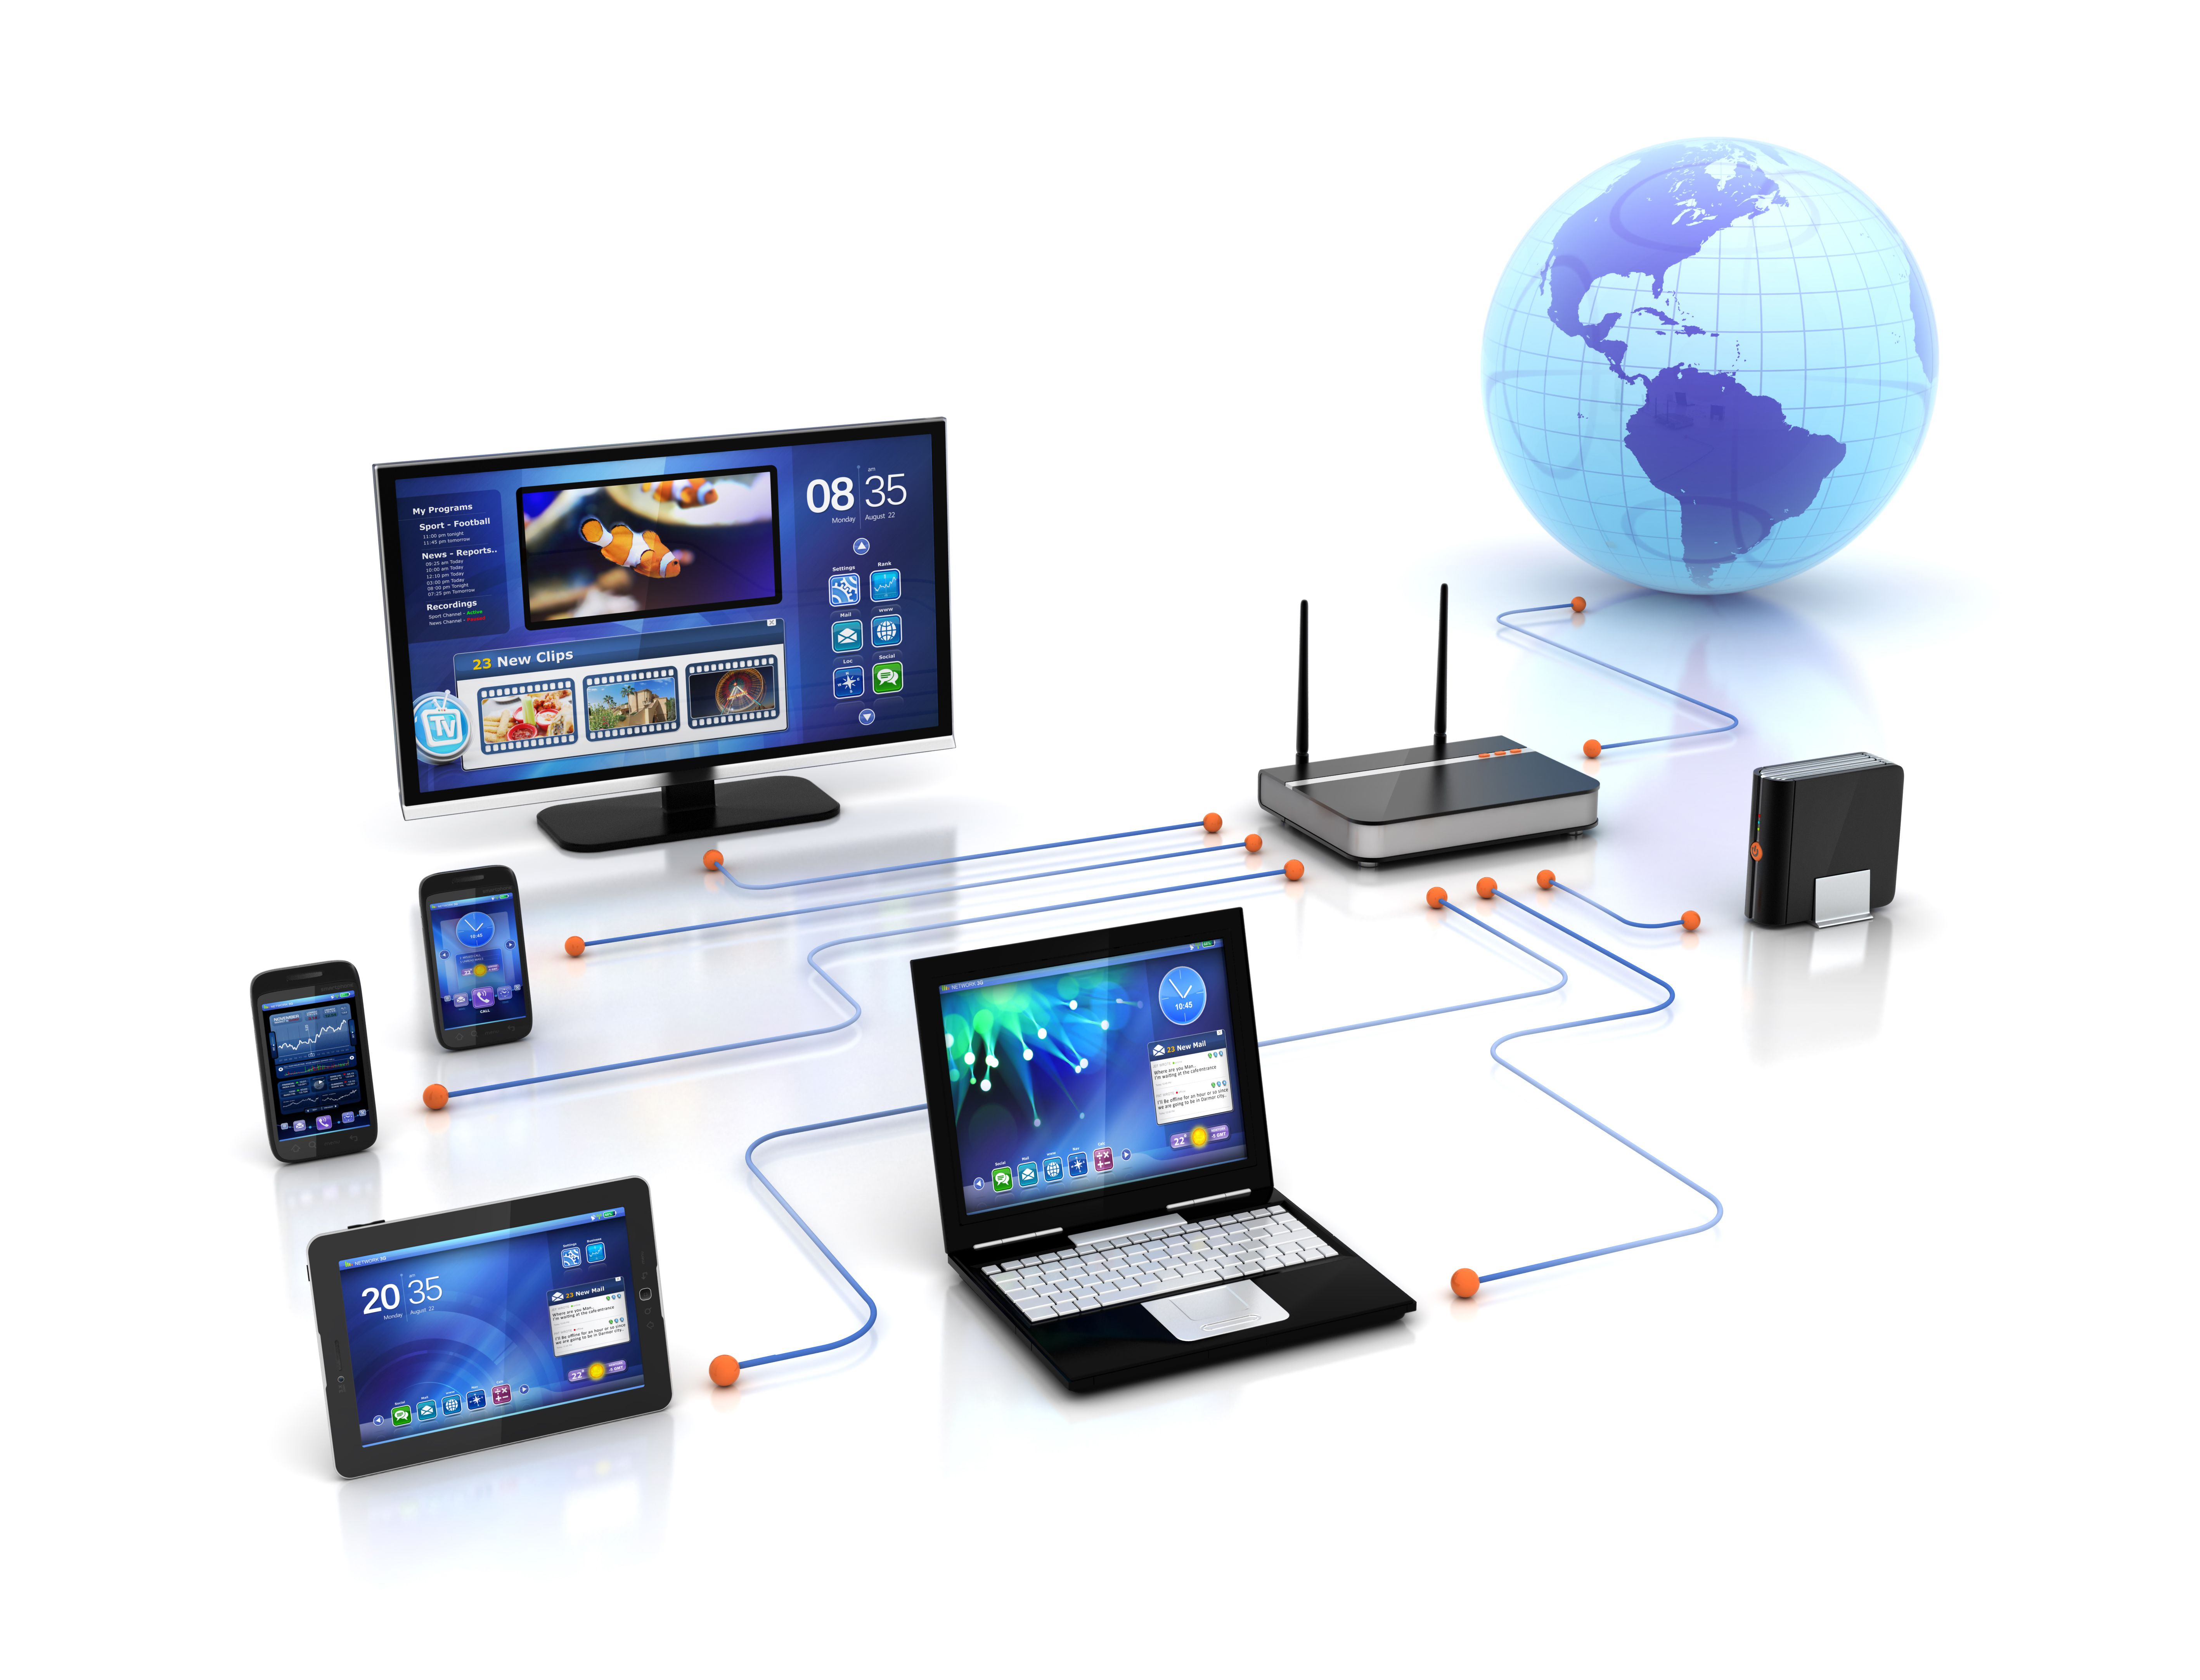
\includegraphics[width=5.1em]{network.jpg}}
\end{picture}
}

\def\LOG{
\begin{picture}(0,0)\unitlength=0.5cm
\put (-6,0) {
\includegraphics[width=4em]{question.png}}
\end{picture}
}

\definecolor{mygreen}{rgb}{0,0.6,0}
\definecolor{mygray}{rgb}{0.5,0.5,0.5}
\definecolor{mymauve}{rgb}{0.58,0,0.82}

\lstset{ 
  backgroundcolor=\color{white},   % choose the background color
  basicstyle=\footnotesize,        % size of fonts used for the code
  breaklines=true,                 % automatic line breaking only at whitespace
  captionpos=b,                    % sets the caption-position to bottom
  commentstyle=\color{mygreen},    % comment style
  keywordstyle=\color{blue},       % keyword style
  stringstyle=\color{mymauve},     % string literal style
}


\begin{document}

\title{\LOG        سوال ۲ کلاس استاد        \LOGO }
\author{نازنین صبری\\۸۱۰۱۹۴۳۴۶}
\date{ ۲۰ اسفند ۱۳۹۶}
\maketitle

\renewcommand{\labelenumii}{\alph{enumii}}
\begin{enumerate}
	\item  پروتکل \lr{FTP} از چه پورت‌هایی استفاده می‌کند؟\\این پروتکل برای انتقال داده از ۲ اتصال \lr{TCP} موازی استفاده می‌کند، یکی اتصال کنترل که روی پرت ۲۱ است و دیگری اتصال داده که روی پرت ۲۰ است. اتصال کنترل برای ارسال اطلاعات کنترلی بین دو میزبان به کار می‌رود، اطلاعاتی مانند شناسه کاربری و گذرواژه، فرمان‌هایی مثل تغییر دایرکتوری در میزبان دور و فرمان جابجا کردن فایل بین دو میزبان اما انتقال واقعی از طریق اتصال داده انجام می‌شود. از آنجا که این پروتکل از یک اتصال کنترل جداگانه استفاده می‌کند گفته می‌شود که مبادله اطلاعات در آن خارج از باند است. 
\end{enumerate}


\end{document}